\clearpage
\title{Problem 7.1}
\author{}
\date{}
\maketitle

\section*{Problem Description}
Reverse an array.

\section*{Tools Used}
\begin{itemize}
    \item emu8086 - 8086 Microprocessor Emulator
    \item MacTeX -\LaTeX  compiler.
    \item VS Code with \LaTeX workshop extension as a text editor.
\end{itemize}

\section*{Process}
\subsection*{Code:}
\begin{multicols}{2}{|}
    \begin{minted}[linenos,breaklines,breakanywhere]{nasm}
DATA SEGMENT
    ARR DB 1, 2, 3, 4, 5, 6, 7, 8
DATA ENDS

CODE SEGMENT
    ASSUME DS:DATA, CS:CODE

START:
    MOV AX, DATA
    MOV DS, AX
    
    MOV CX, 4
    XOR AX, AX
    
    LEA SI, ARR
    MOV DI, SI
    ADD DI, 7

REVERSE:
    MOV AL, [SI]
    XCHG AL, [DI]
    XCHG [SI], AL
    
    INC SI
    DEC DI
    
    LOOP REVERSE

CODE ENDS
END START
    \end{minted}
\end{multicols}


\subsection*{Output}
\begin{center}
    \centering
    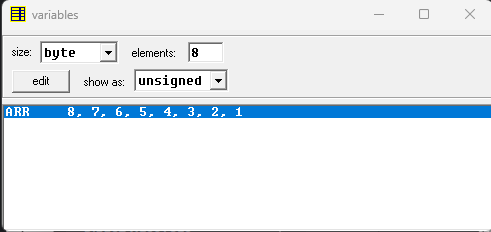
\includegraphics[width = \textwidth]{rev.png}
    \captionof{figure}{Reversed array.}
\end{center}

